\begin{appendix} %Anhang

\begin{landscape}
\section{Motoren im Vergleich}\label{appsec:Motoren}
	\begin{figure}[H]
	\begin{center}
		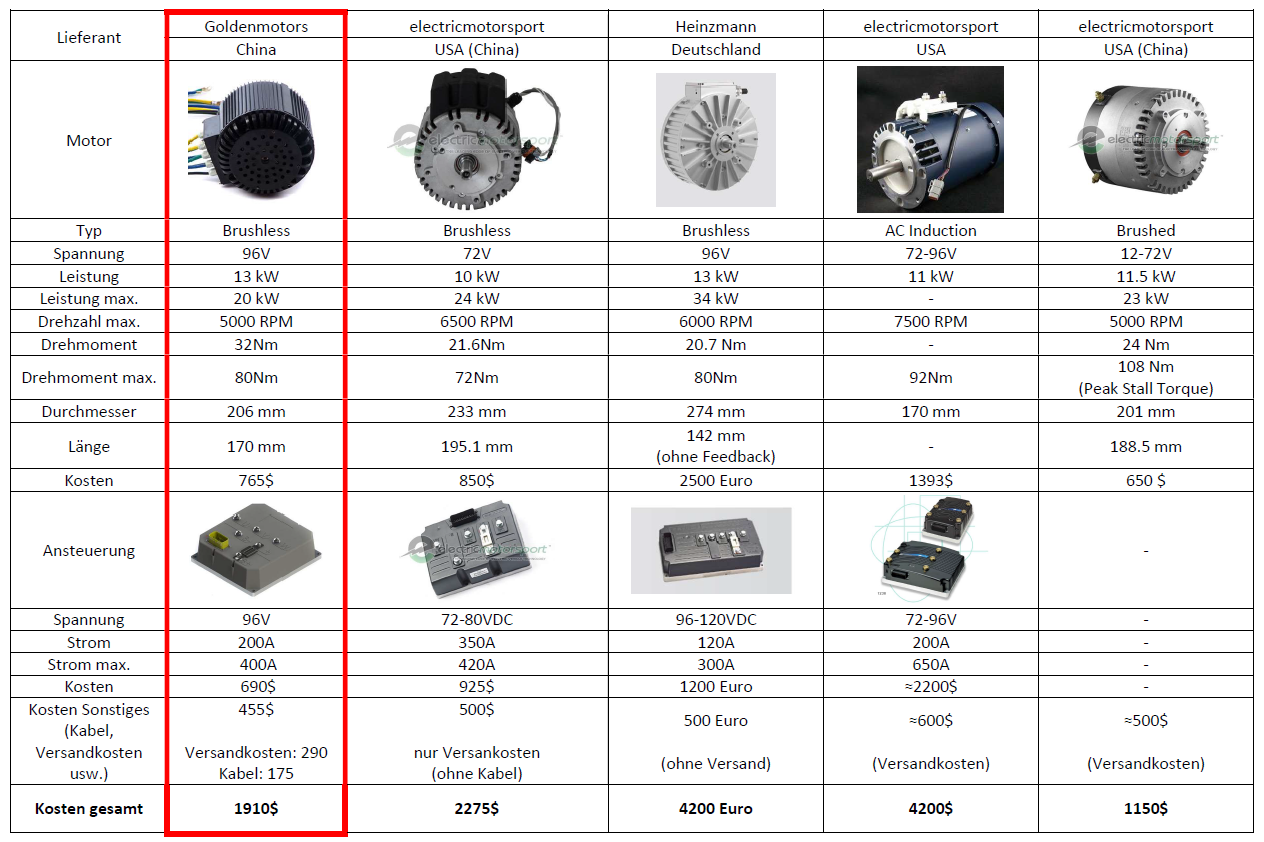
\includegraphics[width=240mm]{appendix/Motoren.png}
		\caption[Motoren im Vergleich]{Motoren im Vergleich} %picture caption
		\label{fig:Motoren}
	\end{center}
\end{figure}
\end{landscape}

	
\begin{landscape}
\section{Batterien im Vergleich}\label{appsec:Batterie}
	\begin{figure}[H]
		\begin{center}
			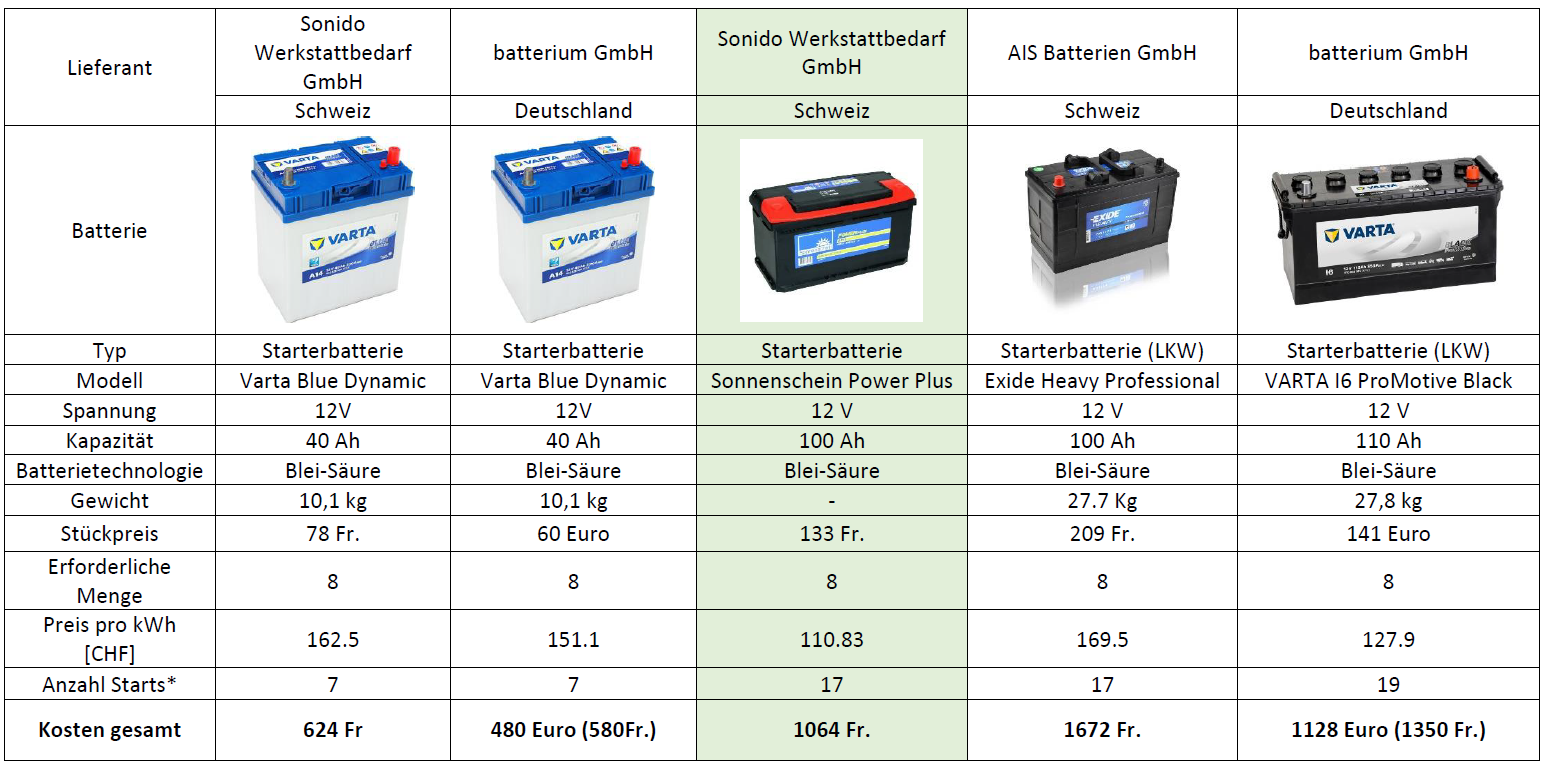
\includegraphics[width=240mm]{appendix/BatterieStart.png}
			\caption[Starterbatterien im Vergleich]{Starterbatterien im Vergleich} %picture caption
			\label{fig:Starterbatterie}
		\end{center}
	\end{figure}

	\begin{figure}[H]
		\begin{center}
			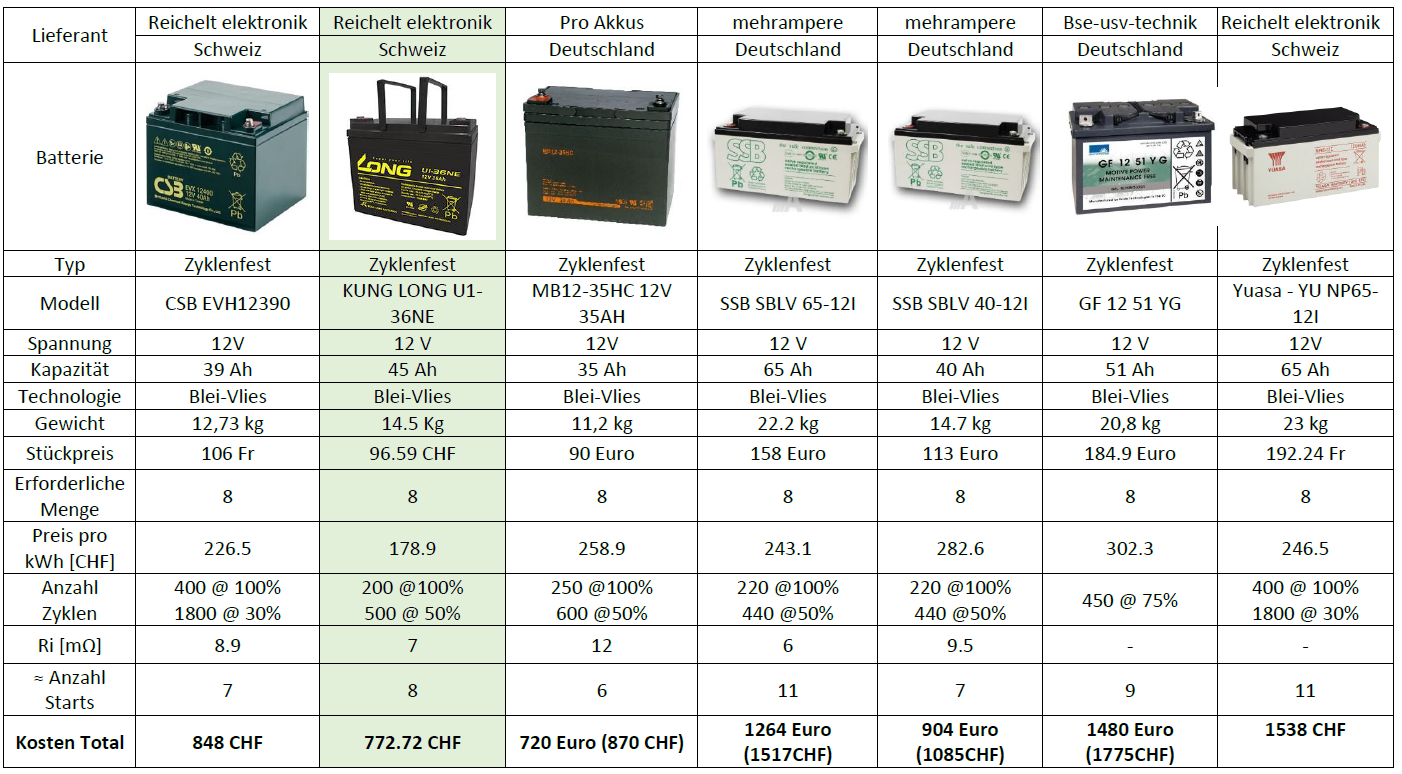
\includegraphics[width=240mm]{appendix/BatterieZyklenfest.png}
			\caption[Zyklenfestebatterien]{Zyklenfestebatterien im Vergleich} %picture caption
			\label{fig:Zyklenfestebatterie}
		\end{center}
	\end{figure}
\end{landscape}


\begin{table}[H]
	\centering
	\begin{tabular}{C{2cm} C{2cm} C{2cm} C{2cm} C{2cm}} 
		\multicolumn{5}{c}{\textbf{Messdaten Kapitel \ref{subsec:DrehmomentDrehzahl}}} \\
		{Strom}& {Spannung} & {Frequenz}& {Leistung}& {Sollwert}\\ \hline\hline 
		37.8 & 96.2 & 40.9 & 1702 & 141\\
		41.7& 96.5& 48.45& 2033& 143\\
		44.7& 96.2& 53.99& 2305& 143\\
		50.1& 96.2& 63.56& 2813& 143\\
		54& 96.3& 66.07& 2930 &141\\
		55.9& 96.2& 73.53& 3232 &143\\
		59.6& 96& 79.11& 3513 &143\\
		63.8& 96.3& 86.22& 3882& 143\\
		67 &96.3& 92.94& 4219& 143\\
		67.7& 96.2& 96.91& 4264& 146\\
		74.8 &96& 100.4& 4598& 143\\
		79 &96& 108.9& 4964& 143\\
		80 &96.2& 113.1& 5065& 143\\
		83.3& 96.3& 119.6& 5421& 142\\
		90.9& 95.9& 127& 5890& 143\\
		93.81& 96.6& 133& 6119& 143\\
		97.1 &96.2& 139.7& 6385& 143\\
		100& 96.4& 146.3& 6631& 143\\
		104& 95.7& 153.4& 6922& 143\\
		107& 96.1& 160.2& 7170& 143\\
		114& 96.5& 167.9& 7651& 141\\
		113& 96.2& 174.8& 7791& 145\\
		117& 96.2& 179.5& 8054& 144\\
		119& 96.2& 186.4& 8287& 144\\
		122& 96.4& 186.3& 8427& 142\\
		125& 96.3& 192.3& 8677& 142\\
		128& 96.1& 196.9& 8870& 142\\
	\end{tabular}
	\caption{Messdaten Drehmoment bei variabler Drehzahl}\label{tab:MessdatenDrehmomentDrehzahl}
\end{table}


\begin{table}[H]
	\centering
	\begin{tabular}{C{2cm} C{2cm} C{2cm}} 
		\multicolumn{3}{c}{\textbf{Messdaten Kapitel \ref{subsec:DrehzahlSpanungsabfall}}} \\
		{Strom}& {Spannung} & {Frequenz}\\ \hline\hline 
		9.33&  64.7& 193.8\\
		9.63&  67& 201.4\\
		9.98&  69.3& 206.6\\
		10.2 & 71.2& 211.9\\
		10.6&  73.2& 217.3\\
		10.8& 75.5& 224.13\\
		11.4& 77.4& 230.8\\
		11.6& 79.6& 235.8\\
		11.5& 81.1& 242.7\\
		11.6& 83.5& 249.7\\
		13.1& 85.8& 252.5\\
		12.1& 87.2& 252.5\\
		10.9& 89.6& 252.0\\
		10.2& 90.7& 252.5\\
	\end{tabular}
	\caption{Messdaten max. Drehzahl bei variabler Spannung}\label{tab:MessdatenDrehzahlSpannung}
\end{table}

\begin{table}[H]
	\centering
	\begin{tabular}{C{2cm} C{2cm} C{2cm} C{2cm}} 
		\multicolumn{4}{c}{\textbf{Messdaten Kapitel \ref{subsec:LeistungSpannungabfall}}} \\
		{Strom}& {Spannung} &{Frequenz} & {Leistung}\\ \hline\hline 
		9.94& 80.1& 238& 23\\
		13.9& 80.6& 238& 100\\
		17.8& 81.2& 238.1& 380\\
		22& 81.7& 238.1& 710\\
		26.3& 82.2& 238.1& 1060\\
		30.2& 82.7& 238.1& 1350\\
		33.8& 83.2& 238.1& 1630\\
		38.2& 83.7& 238& 1940\\
		42.9& 84.2& 238.1& 2310\\
		47.6& 84.8& 238.1& 2650\\
		51.6& 85.2& 238& 2990\\
		56.6& 85.6& 238.1& 3370\\
		62.4& 86.2& 238.1& 3780\\
		68.6& 86.4& 238.1& 4122\\
		67.1& 86.6& 238.1& 4250\\
		73.3& 87.1& 238& 4600\\
		80.1& 87.7& 238.1& 5138\\
		85.5& 88.1& 238& 5520\\
		92.7& 88.7& 238& 6150\\
		99.3& 89.3& 238& 6603\\
		100& 89.2& 238& 6666\\
	\end{tabular}
	\caption{Messdaten max. Leistung bei variabler Spannung}\label{tab:MessdatenLeistungSpannung}
\end{table}


\begin{table}[H]
	\centering
	\begin{tabular}{C{2cm} C{2cm} C{2cm}} 
		\multicolumn{3}{c}{\textbf{Messdaten Kapitel \ref{subsec:Temperatur} (Erwärmung)}} \\
		{Temperatur}& {Zeit (1550 RPM)} & {2550 RPM}\\ \hline\hline 
		55& 19.9 &20.92\\
		60& 48.07 &49.9\\
		65& 81.16 &81\\
		70& 114.09 &107.17\\
		75& 139.63 &135.93\\
		80& 179.87& 171.66\\
		85& 216.35& 205.21\\
		90& 252.17& 235.56\\
		95& 319& 292.12\\
		100& 372.7&338.29\\
	\end{tabular}
	\caption{Messdaten Temperatur in Abhängigkeit der Drehzahl}\label{tab:MessdatenTemperatur}
\end{table}

\begin{table}[H]
	\centering
	\begin{tabular}{C{3cm} C{3cm} C{3cm} C{3cm}} 
		\multicolumn{4}{c}{\textbf{Messdaten Kapitel \ref{subsec:Temperatur} (Motor)}} \\
		{Zeit}& {Temperatur} & {Zeit}& {Temperatur}
		(1 Venitaltor)&(1 Venitaltor)&(3 Venitaltor)&(3 Venitaltor)\\
		\\ \hline\hline 
		0    & 45  & 0    & 40  \\
		26   & 50  & 20   & 45  \\
		46   & 55  & 52   & 50  \\
		70   & 60  & 80   & 55  \\
		100  & 65  & 117  & 60  \\
		129  & 70  & 153  & 65  \\
		161  & 75  & 183  & 70  \\
		195  & 80  & 214  & 75  \\
		235  & 85  & 263  & 80  \\
		269  & 90  & 295  & 85  \\
		343  & 95  & 340  & 90  \\
		410  & 100 & 399  & 95  \\
		448  & 100 & 455  & 100 \\
		517  & 95  & 483  & 100 \\
		560  & 90  & 520  & 95  \\
		634  & 85  & 570  & 90  \\
		690  & 80  & 628  & 85  \\
		765  & 75  & 675  & 80  \\
		888  & 70  & 730  & 75  \\
		1020 & 65  & 816  & 70  \\
		1207 & 60  & 908  & 65  \\
		1500 & 55  & 1008 & 60  \\
		1825 & 50  & 1170 & 55  \\
		-    & -   & 1342 & 50  \\
	\end{tabular}
	\caption{Messdaten Temperatur des Motors}\label{tab:MessdatenTemperaturMotor}
\end{table}



\begin{table}[H]
	\centering
	\begin{tabular}{C{3cm} C{3cm} C{3cm} C{3cm}} 
		\multicolumn{4}{c}{\textbf{Messdaten Kapitel \ref{subsec:Temperatur} (Controller)}} \\
		{Zeit}& {Temperatur} & {Zeit}& {Temperatur}\\
		(mit Kühlkörper)&(mit Kühlkörper)&(ohne Kühlkörper)&(ohne Kühlkörper)\\ \hline\hline 
		0    & 38 & 73   & 34 \\
		15   & 41 & 100  & 36 \\
		40   & 44 & 125  & 38 \\
		58   & 46 & 140  & 40 \\
		80   & 47 & 170  & 42 \\
		103  & 49 & 190  & 44 \\
		134  & 51 & 207  & 46 \\
		175  & 53 & 243  & 48 \\
		208  & 55 & 267  & 50 \\
		250  & 57 & 286  & 52 \\
		304  & 59 & 315  & 54 \\
		354  & 62 & 345  & 56 \\
		425  & 64 & 367  & 58 \\
		472  & 62 & 400  & 60 \\
		485  & 59 & 415  & 62 \\
		517  & 57 & 446  & 64 \\
		554  & 55 & 538  & 62 \\
		599  & 53 & 630  & 60 \\
		648  & 51 & 739  & 58 \\
		708  & 49 & 864  & 56 \\
		765  & 47 & 1005 & 53 \\
		823  & 46 & 1144 & 51 \\
		888  & 44 & 1322 & 49 \\
		953  & 43 & -    & -  \\
		1033 & 41 & -    & -  \\
		1108 & 40 & -    & -  \\
		1193 & 39 & -    & -  \\
		1288 & 38 & -    & -  \\
		1308 & 37 & -    & -  \\
		1392 & 36 & -    & -  \\
		1503 & 35 & -    & -  \\
		1645 & 34 & -    & -  \\
		1765 & 33 & -    & -  \\
	
	\end{tabular}
	\caption{Messdaten Temperatur des Controllers}\label{tab:MessdatenTemperaturContorller}
\end{table}



\end{appendix}
